\subsection{Строение и состав ионосферы. Процессы в ионосфере. Чепменовский слой.}
\textit{Ионосфера} -- это область верхней атмосферы Земли на высотах примерно от 60 км до 1000 км и более, в которой длительное время могут существовать свободные электроны.

Главным механизмом образования свободных электронов в ионосфере является ионизация.
\textit{Ионизация} – это процесс, при котором электрически нейтральный атом или молекула теряет либо приобретает электрон, что приводит к образованию положительного или отрицательного иона, соответственно.
В верхних слоях атмосферы высокоэнергичные солнечные фотоны сталкиваются с частицами газа, лишают их электронов и ионизируют их.
Этот процесс называется \textit{фотоионизацией}.

Если бы свободные электроны, образованные из-за фотоионизации, не исчезали бы под воздействием каких-либо процессов, их количество в ионосфере необратимо возрастало бы.
Поэтому существует обратный процесс -- \textit{рекомбинация}.

На малых высотах наиболее распространены ионы $O^+_2$, $N^+_2$ и $NO^+$.
Эти молекулярные ионы доминируют примерно до 200 км, после чего доминирующим ионом становится $O^+$.
На высотах более 700 км количество ионов $O^+$ начинает уменьшаться и на их место приходят ионы $H^+$ и $He^+$.

Строение ионосферы (см. рис. \ref{fig:ne(h)}):
\begin{enumerate}
\item Слой D (60 -- 90 км).
\item Слой E (90 -- 140 км).
\item Спарадический слой Es -- слой на высоте примерно 100 км, в котором преобладают ионы металлов метеорного происхождения.
\item Слой F1 (140 -- 210 км).
\item Слой F2 (210 -- 600 км).
\end{enumerate}

\begin{figure}[!ht]
\centering
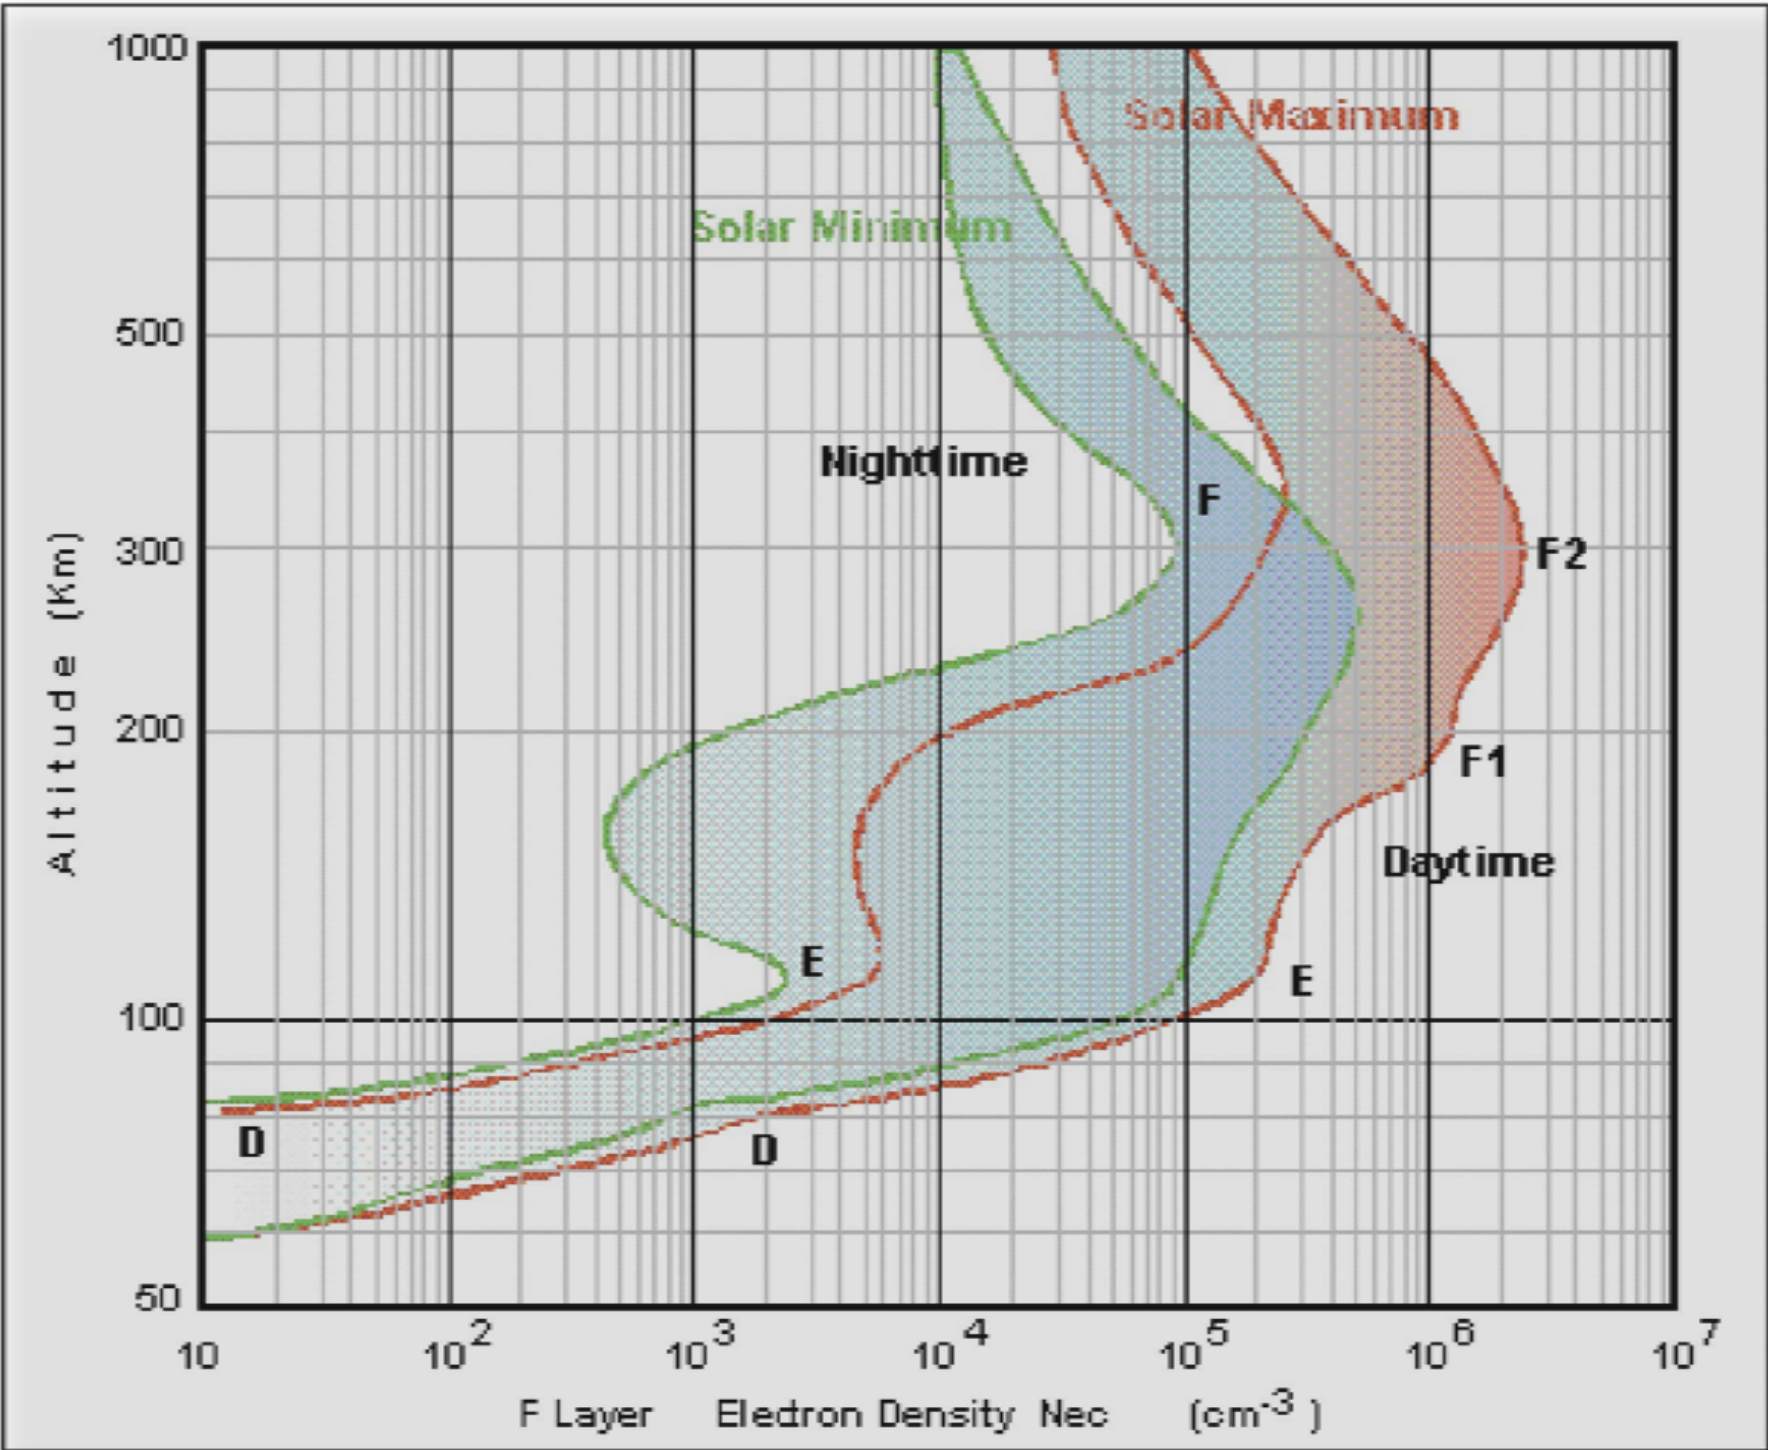
\includegraphics[width=0.4\textwidth]{images/ne(h).png}
\caption{Профиль электронной концентрации ионосферы.}\label{fig:ne(h)}
\end{figure}

Чепменовский слой -- математическая модель ионосферного\footnote{Изначально Чепменовский слой разрабатывался для озонового слоя.} слоя, которая представляет собой суперпозицию между концентрацией нейтралов (барометрическим законом) и интенсивностью солнечного излучения (законом Бугера) (см. рис. \ref{fig:chap}):
\begin{equation}
n_e=n_0 e^{k\left(1-z-e^{-z}\right)}
\end{equation}
где $z=\frac{h-h_0}{H}$, $n_0$ -- максимальная электронная концентрация на высоте $h_0$, $k=\frac{1}{2}$ -- $\alpha$--Чепменовский слой, $k=1$ -- $\beta$--Чепменовский слой.

\begin{figure}[!ht]
\centering
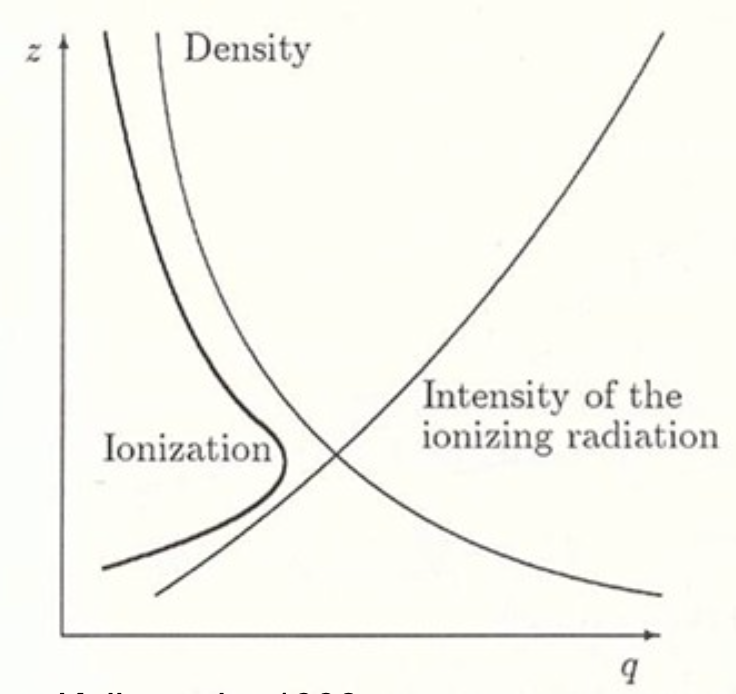
\includegraphics[width=0.4\textwidth]{images/chap.png}
\caption{Модель Чепменовского слоя.}\label{fig:chap}
\end{figure}
